\documentclass[12pt]{article}
\usepackage[a4paper, portrait, margin=1cm, bottom=2cm]{geometry}
\usepackage{fontspec}
\usepackage[fleqn]{amsmath}
\usepackage{amssymb}
\usepackage{graphicx}
\usepackage{indentfirst}
\usepackage{polyglossia}
\usepackage[dvipsnames]{xcolor}
\usepackage{svg}

\setmainfont[Ligatures=TeX]{Linux Libertine O}
\setdefaultlanguage{russian}
\setotherlanguages{english}
\graphicspath{graphics}

\begin{document}
\section{Бесконечные цепные дроби}
$\alpha = [a_0,a_1,...,a_n,...] \vspace{1 ex}$

$ a_0 + \frac{1}{a_1 + \frac{1}{... + \frac{1}{a_n + \frac{1}{a\textsubscript{n+1} + ...}}}} = \alpha \vspace{1 ex}$

$..+ \frac{1}{a_n + \frac{1}{a\textsubscript{n+1} + ...}} = \eta_n \vspace{2 ex}$

$\eta_n = [a_n,a\textsubscript{n+1}, a\textsubscript{n+1}, ...] \rightarrow \alpha = [a_0,a_1,...,\eta_n]  \vspace{2 ex}$

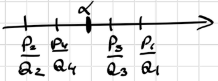
\includegraphics[width=30mm]{image.png}

$! \hspace{2 ex} \alpha$ между $\frac{P_s}{Q_s}$ и $\frac{P\textsubscript{s+1}}{Q\textsubscript{s+1}} $

Доказательство:

$\alpha = \frac{P_n}{Q_n} = \frac{\eta_n P\textsubscript{n-1} + P\textsubscript{n-2}}{\eta_n Q\textsubscript{n-1} + Q\textsubscript{n-2}} \vspace{2 ex}$

$1) \alpha - \frac{P\textsubscript{n-1}}{Q\textsubscript{n-1}} = \frac{\eta_n P\textsubscript{n-1} + P\textsubscript{n-2}}{\eta_n Q\textsubscript{n-1} + Q\textsubscript{n-2}} - \frac{P\textsubscript{n-1}}{Q\textsubscript{n-1}} 
= \frac{\eta_n P\textsubscript{n-1} Q\textsubscript{n-1} + P\textsubscript{n-2} Q\textsubscript{n-1} - \eta_n P\textsubscript{n-1} Q\textsubscript{n-1} - P\textsubscript{n-1} Q\textsubscript{n-2}}{ Q\textsubscript{n-1}(\eta_n Q\textsubscript{n-1} + Q\textsubscript{n-2})} = \vspace{2 ex}$

$\frac{(-1)^n^-^1}{Q\textsubscript{n-1}(\eta_n Q\textsubscript{n-1} + Q\textsubscript{n-2})} \vspace{2 ex}$

$2) \alpha - \frac{P\textsubscript{n-2}}{Q\textsubscript{n-2}} = \frac{\eta_n P\textsubscript{n-1} + P\textsubscript{n-2}}{\eta_n Q\textsubscript{n-1} + Q\textsubscript{n-2}} - \frac{P\textsubscript{n-2}}{Q\textsubscript{n-2}} 
= \frac{\eta_n P\textsubscript{n-1} Q\textsubscript{n-2} + P\textsubscript{n-2} Q\textsubscript{n-2} - \eta_n P\textsubscript{n-2} Q\textsubscript{n-1} - P\textsubscript{n-2} Q\textsubscript{n-2}}{ Q\textsubscript{n-2}(\eta_n Q\textsubscript{n-1} + Q\textsubscript{n-2})} = \vspace{2 ex}$

$ = \frac{\eta_n (P\textsubscript{n-1} Q\textsubscript{n-2} - P\textsubscript{n-2} Q\textsubscript{n-1})}{Q\textsubscript{n-2}(\eta_n Q\textsubscript{n-1} + Q\textsubscript{n-2}) }
= \frac{\eta_n (-1)^n^-^2}{Q\textsubscript{n-2}(\eta_n Q\textsubscript{n-1} + Q\textsubscript{n-2})}
\vspace{2 ex}$

$ 3)
|\alpha - \frac{P\textsubscript{n-1}}{Q\textsubscript{n-1}}| = \frac{Q\textsubscript{n-2}}{\eta_n Q\textsubscript{n-1}} (< 1) |\alpha - \frac{P\textsubscript{n-2}}{Q\textsubscript{n-2}}| \hspace{2 ex}
Q\textsubscript{n-2} < Q\textsubscript{n-1} \leq \eta_n Q\textsubscript{n-1} |\rightarrow |\alpha - \frac{P\textsubscript{n-1}}{Q\textsubscript{n-1}}| < |\alpha - \frac{P\textsubscript{n-2}}{Q\textsubscript{n-2}}| 
\vspace{2 ex}$

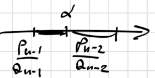
\includegraphics[width=30mm]{image1.png}
$\rightarrow$ Следствие:$ |\alpha - \frac{P\textsubscript{n}}{Q\textsubscript{n}}| < \frac{1}{Q^2_n}$

Доказательство: $|\alpha - \frac{P\textsubscript{n}}{Q\textsubscript{n}}| \leq |\frac{P\textsubscript{n+1}}{Q\textsubscript{n+1}} - \frac{P\textsubscript{n}}{Q\textsubscript{n}}| = \frac{1}{Q_n Q\textsubscript{n+1}} < \frac{1}{Q^2_n}  \vspace{2 ex}$

$Q\textsubscript{n+1} > Q_n$

$\frac{1}{Q\textsubscript{n+1}} < \frac{1}{Q_n} $

Пример:
$\sqrt{28} = 5 + (\sqrt{28} -5) = 5 + \frac{1}{\frac{1}{\sqrt{28} - 5}} = 5 + \frac{1}{\frac{\sqrt{28} + 5}{3}} =  5 + \frac{1}{3 + \frac{\sqrt{28}-4}{3}} = 5 + \frac{1}{3 + \frac{1}{\frac{3}{\sqrt{28}-4}}} \vspace{1 ex}$

$\frac{3}{\sqrt{28} -4} = \frac{3(\sqrt{28} + 4)}{12} = 2 + \frac{\sqrt{28} - 4}{4} =|\frac{4}{\sqrt{28} - 4} \frac{\sqrt{28} + 4}{3} = 3 + \frac{\sqrt{28} - 5}{3}| \vspace{1 ex}$

$\frac{3}{\sqrt{28} -5} = \sqrt{28} + 5 = 10 (\sqrt{28} - 5)...$ итого: $\sqrt{28} = [5;3,2,3,10] = [5;(3,2,3,10)]$

\section{Цепные дроби. Непр. дроби}

$[a_0,a_1,a_2,...,a_n] = a_0 + \frac{1}{a_1 + \frac{1}{a_2 + \frac{1}{... + \frac{1}{a_n}}}}; a_0 \in Z; a_1,...,a_n \in N; a_n > 1
\vspace{1 ex}$

$\frac{a}{b} = q_1 + \frac{r_1}{b} = q_1 + \frac{1}{\frac{b}{r_1}} = q_1 + \frac{1}{q_2 + \frac{r_2}{r_1}} = ... = [q_1,q_2,q_3,...,q\textsubscript{k+1}] \vspace{2 ex}$

$-\frac{48}{109} = [-1,1,1,3,1,2,4] $

$-48 = 109(-1) + 61$

$109 = 61*1 +48$

$61 = 48*1 + 13$

$48 = 13*3 + 9$

$13 = 9*1 + 4$

$9 = 4*2+1$

$4=1*4$

$\alpha = [a_0,a_1,...,a_n]$

Подходящая дробь

$\delta_k = [a_0,a_1,...,a_k]$

$\delta_0 = [-1] = \frac{P_0}{Q_0}$

$\delta_1 = [-1,1] = \frac{P_1}{Q_1}$

$\delta_2 = [-1,1,1] = \frac{P_2}{Q_2}$

$\delta_3 = [-1,1,1,3] = \frac{P_3}{Q_3}$

$P_0 = Q_0 \hspace{1 ex } Q_0 = 1$

$\delta_0 = [a_0] = \frac{a_0}{0} = \frac{P_0}{Q_0}$

$\delta_1 = [a_0, a_1] = a_0 + \frac{1}{a_1} = \frac{a_0 a_1 +1}{a_1} \hspace{2 ex} P_1 = a_0 a_1 +1 \hspace{1 ex} Q_1 = a_1$

$\delta_k = [a_0,a_1,...,a_k] = \frac{P_k(a_0,...,a_k)}{Q_k(a_0,..,a_k)}$

$\delta\textsubscript{k+1} = [a_0,a_1,...,a_k,a\textsubscript{k+1}] =[a_0,a_1,...,a_k+\frac{1}{ a\textsubscript{k+1}}] =  \frac{P_k(a_0,...,a_k+\frac{1}{ a\textsubscript{k+1}} )}{Q_k(a_0,..,a_k+\frac{1}{ a\textsubscript{k+1}})} = \vspace{2 ex}$

$= \frac{(a_k + \frac{1}{a\textsubscript{k+1}}) P\textsubscript{k-1} + P\textsubscript{k-2}}{(a_k + \frac{1}{a\textsubscript{k+1}}) Q\textsubscript{k-1} + Q\textsubscript{k-2}} =
= \frac{a_k q\textsubscript{k+1} P\textsubscript{k-1} + P\textsubscript{k-1} + q\textsubscript{k+1} P\textsubscript{k-2}}{a_k q\textsubscript{k+1} Q\textsubscript{k-1} + Q\textsubscript{k-1} + q\textsubscript{k+1} P\textsubscript{k-2}} = \frac{a\textsubscript{k+1} (a_k P\textsubscript{k-1} + P\textsubscript{k-2}) + P\textsubscript{k-1}}{a\textsubscript{k+1} (a_k Q\textsubscript{k-1} + Q\textsubscript{k-2}) + Q\textsubscript{k-1}} = $

$= \frac{a\textsubscript{k+1} P_k + P\textsubscript{k-1}}{a\textsubscript{k+1} Q_k + Q\textsubscript{k-1}} = \frac{P\textsubscript{k+1}}{Q\textsubscript{k+1}} \hspace{2 ex} P\textsubscript{k+1} = a\textsubscript{k+1} P_k + P\textsubscript{k-1} ; \hspace{2 ex} Q\textsubscript{k+1} = a\textsubscript{k+1} Q_k + Q\textsubscript{k-1} \vspace{2 ex}$


$\delta_2 = [a_0,a_1,a_2] = a_0 + \frac{1}{a_1 + \frac{1}{a_2}} = a_0 + \frac{a_2}{a_1 a_2 + 1} = \frac{a_0 a_1 a_2 + a_0 + a_2}{a_1 a_2 + 1}$

$P_2 = a_0 a_1 a_2 + a_0 + a_3$

$Q_2 = a_1 a_2 +1$

$[-1;1,1,3,1,2,4]$

$k \hspace{1 ex} -1\hspace{2 ex}0\hspace{2 ex}1\hspace{2 ex}2\hspace{2 ex}3\hspace{2 ex}4\hspace{2 ex}5\hspace{2 ex}6$

$a_n  \hspace{1 ex}\hspace{2 ex}-1\hspace{2 ex}1\hspace{2 ex}1\hspace{2 ex}3\hspace{2 ex}1\hspace{2 ex}2\hspace{2 ex}4$

$P_n \hspace{2 ex} 1-1\hspace{2 ex}0-1-3-4-11-48$

$Q_n \hspace{2 ex} 0\hspace{2 ex}1\hspace{2 ex}1\hspace{2 ex}2\hspace{2 ex}7\hspace{2 ex}9\hspace{2 ex}25\hspace{2 ex}109$

$\delta_0 = -1; \delta_1 = 0; \delta_2 = -\frac{1}{2} ;\delta_3 = -\frac{3}{7} ; \delta_4 =-\frac{4}{9} ; \delta_5 = -\frac{11}{25} ; \delta_6 = \alpha = -\frac{48}{109}$

Утв. $\frac{P_s}{Q_s} - \frac{P\textsubscript{s-1}}{Q\textsubscript{s-1}} = \frac{(-1)^s^+^1}{Q_s Q\textsubscript{s-1}}$

Док-во: $\frac{P_s}{Q_s} - \frac{P\textsubscript{s-1}}{Q\textsubscript{s-1}} = \frac{P_s Q\textsubscript{s-1} - P\textsubscript{s-1} Q_s}{Q_s Q\textsubscript{s-1}}$

$h_s = P_s Q\textsubscript{s-1} - P\textsubscript{s-1} Q_s = (a_s P\textsubscript{s-1} + P\textsubscript{s-2}) Q\textsubscript{s-1} - P\textsubscript{s-1}(a_s Q\textsubscript{s-1} + Q\textsubscript{s-2}) = P\textsubscript{s-2} Q\textsubscript{s-1} - P\textsubscript{s-1} Q\textsubscript{s-2} = $


$= -(P\textsubscript{s-1} Q\textsubscript{s-2} - P\textsubscript{s-2} Q\textsubscript{s-1} ) = -h\textsubscript{s-1} = h\textsubscript{s-2} = -h\textsubscript{s-3} = ... = (-1)^s^-^1 h_1 =(-1)^s^-^1 (P_1 Q_0 - P_0 Q_1) =  (-1)^s^-^1 (a_0 a_1 +1 - a_0 a_1) = (-1)^s^-^1$

Следствие: НОД$(P_s, Q_s) = 1$ (все подходящие дроби несократимы/ взаим. просты)

Следствие: $\lim_{s \to \infty}|\frac{P_s}{Q_s} - \frac{P\textsubscript{s-1}}{Q\textsubscript{s-1}}| = 0$ (последов. подходящ. дробей фундамент.)

\section{Науилучшие приближения}
$|\alpha - \frac{x}{y}|$

Опр.$\frac{a}{b}$ - наилучш. приближ. к числу $\alpha$, если не сущ. другой дроби $\frac{x}{y}: 
\begin{cases}
    $|\alpha - \frac{x}{y}| \leq |\alpha - \frac{a}{b}|$ \\
    0 < y < b              
\end{cases}
$

Утв. $\frac{x}{y} \in (\frac{a}{b}; \frac{c}{d})$ и $bc- ad = 1 \rightarrow y > b $ и $y>d$

Доказательство: $\frac{c}{d} - \frac{a}{b} = \frac{bc - ad}{bd} = \frac{1}{bd}$ (по услов.)

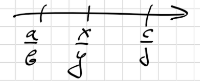
\includegraphics[width=30mm]{image2.png}

$\vspace{2 ex}$

$\frac{bx - ay}{by} = \frac{x}{y} - \frac{a}{b} \leq \frac{1}{bd} |bdy ; \hspace{2 ex} xbd - ady < y; \hspace{2 ex} d \leq (bx - ay)d < y $

$xbd \leq (ad+1)y ; \hspace{2 ex} y \geq \frac{xbd}{ad+1} ;\hspace{2 ex} cy - dx \geq 1$

$0 < \frac{c}{d} - \frac{x}{y} < \frac{1}{bd} ;\hspace{2 ex} 0< \frac{cy - dx}{dy} < \frac{1}{bd} (\frac{cy - dx}{dy} \leq \frac{1}{dy}); \hspace{2 ex} \frac{1}{dy} < \frac{1}{bd} ; b<y$

Следствие: $\alpha \in (\frac{a}{b};\frac{c}{d})$ и $dc - ad = 1 \rightarrow$ та из $(\frac{a}{b}, \frac{c}{d})$, кто ближе к $\alpha$ - наилю приближение.

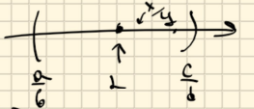
\includegraphics[width=30mm]{image3.png}

Следствие: $\frac{P_s}{Q_s} $ - наил. прибл к $\alpha$

$\frac{P\textsubscript{s-1}}{Q\textsubscript{s-1}}$ и $\frac{P_s}{Q_s} : P\textsubscript{s-1} Q_s - P_s Q\textsubscript{s-1}$
\end{document}